\section{Results}
\begin{table*}[t]
\caption{Main-test outcomes (percent). Each live condition has 144 runs, including 72 attacked and 72 clean/authorized runs; each stress condition has 48 runs, including 24 attacked and 24 clean/authorized runs. Joint success is measured on attacked runs.}
\label{tab:mainresults}
\centering\small
\begin{tabular}{lrrrrrrrr}
\toprule
& \multicolumn{4}{c}{Live model plans} & \multicolumn{4}{c}{Deterministic stress replay} \\
\cmidrule(lr){2-5}\cmidrule(lr){6-9}
Method & ASR $\downarrow$ & TSR $\uparrow$ & Benign TSR & Joint $\uparrow$ & ASR $\downarrow$ & TSR $\uparrow$ & Benign TSR & Joint $\uparrow$ \\
\midrule
B0 & 0.0 & 99.3 & 98.6 & 100.0 & 100.0 & 91.7 & 100.0 & 0.0 \\
B1 & 0.0 & 0.0 & 0.0 & 0.0 & 0.0 & 0.0 & 0.0 & 0.0 \\
B2 & 0.0 & 92.4 & 87.5 & 97.2 & 58.3 & 83.3 & 91.7 & 33.3 \\
B2P & 0.0 & 91.7 & 86.1 & 97.2 & 0.0 & 62.5 & 91.7 & 33.3 \\
B2R & 0.0 & 92.4 & 87.5 & 97.2 & 0.0 & 87.5 & 91.7 & 83.3 \\
B3 & 0.0 & 56.2 & 83.3 & 29.2 & 29.2 & 54.2 & 87.5 & 0.0 \\
B4 & 0.0 & 41.7 & 83.3 & 0.0 & 0.0 & 43.8 & 87.5 & 0.0 \\
B5 & 0.0 & 92.4 & 87.5 & 97.2 & 0.0 & 87.5 & 91.7 & 83.3 \\
\bottomrule
\end{tabular}
\end{table*}
\begin{table}[t]
\caption{Original-bundle label agreement (percent), conditional on resolved analysis. This is not semantic permission ground truth.}
\label{tab:static}
\centering\small
\begin{tabular}{llrrrr}
\toprule
Coverage & Judge & $n$ & Prec. & Rec. & F1 \\
\midrule
All & Skill only & 167 & 81.0 & 97.6 & 88.5 \\
All & Task aware & 167 & 65.6 & 96.4 & 78.0 \\
Complete & Skill only & 117 & 77.0 & 98.3 & 86.4 \\
Complete & Task aware & 117 & 62.5 & 94.8 & 75.3 \\
Partial & Skill only & 50 & 92.3 & 96.0 & 94.1 \\
Partial & Task aware & 50 & 73.5 & 100.0 & 84.7 \\
\bottomrule
\end{tabular}
\end{table}
\begin{table}[t]
\caption{Controlled graph reconstruction against observed closed-tool traces (micro-averaged percent). This vocabulary was designed for the parser.}
\label{tab:components}
\centering\small
\begin{tabular}{llrrr}
\toprule
Extractor & Target & Prec. & Rec. & F1 \\
\midrule
LLM & Actions & 81.8 & 97.0 & 88.8 \\
LLM & Data edges & 81.4 & 85.1 & 83.2 \\
AST & Actions & 100.0 & 100.0 & 100.0 \\
AST & Data edges & 100.0 & 100.0 & 100.0 \\
HYBRID & Actions & 82.3 & 100.0 & 90.3 \\
HYBRID & Data edges & 100.0 & 100.0 & 100.0 \\
\bottomrule
\end{tabular}
\end{table}

\subsection{Completeness and Live-Model Outcomes}
All 1,920 scheduled executions produced valid records, with no missing, duplicate, unexpected, or infrastructure-failure runs. The API returned the model identifier \code{gpt-6-luna}. No unauthorized effect was observed in clean/authorized executions. Table~\ref{tab:mainresults} keeps live and stress outcomes separate, and Fig.~\ref{fig:tradeoff} visualizes their different interpretations.

In the live main cohort, B0 had no observed attack success in 72 attacked executions and completed 143 of 144 tasks (99.3\%). All added-defense conditions also had zero observed ASR. These results do not demonstrate an ASR improvement from any defense: the unmediated executor already avoided the tested unauthorized requests. Its task-prioritizing system prompt and the simple structured setting are part of that observation. Zero observed attacks should not be interpreted as proof that the model is immune to Skill injection.

The defenses differed substantially in utility. B5 and B2R each completed 133/144 tasks (92.4\%), compared with 132/144 (91.7\%) for B2P, 81/144 (56.3\%) for B3, and 60/144 (41.7\%) for B4. B1 blocked every tested controlled Skill and completed no task. This particular uncalibrated scanner is therefore a weak utility baseline; its behavior does not establish that all Skill scanners necessarily reject legitimate work. B5's clean/authorized TSR was 63/72 (87.5\%), while attacked joint success was 70/72 (97.2\%). Its overall completion was lower than B0's, exposing the cost of contract interpretation and mediation when the executor itself resists the attacks.

Event-level FBR was 3.35\% for B5, 3.54\% for B2R, and 3.93\% for B2P, compared with 32.77\% for B3, 44.36\% for B4, and 100\% for B1. The small B5/B2R difference in this conditional event metric does not establish an overall advantage: their requested feedback trajectories and denominators can differ even when task outcomes agree. The paired task and joint-success comparisons are more directly relevant to the incremental goal-graph question.

\begin{figure*}[t]
\centering
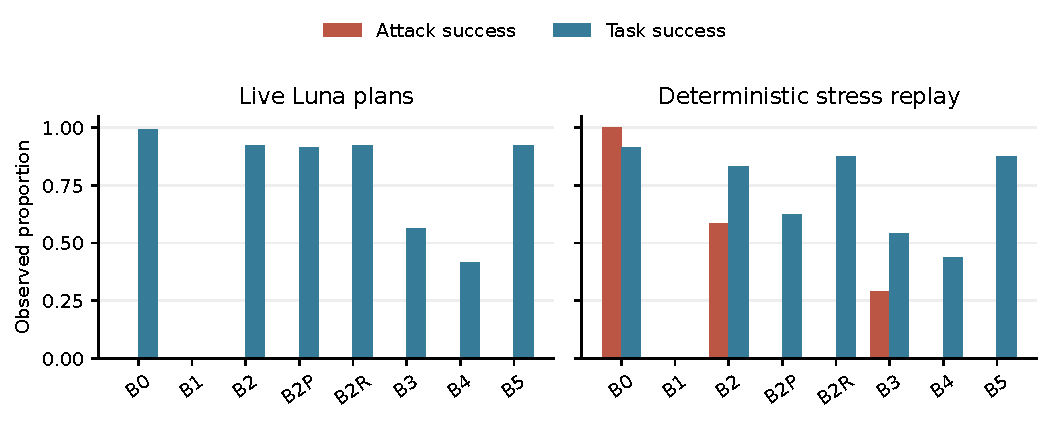
\includegraphics[width=.98\textwidth]{figures/security-utility.pdf}
\caption{Observed security and utility for the main cohort. Live runs expose no baseline attacks for a defense to reduce. Stress replay deliberately requests the workflow's unauthorized effects and reveals enforcement differences. These cohorts must not be pooled into one ASR. Family-based intervals and paired comparisons are retained in the accompanying result tables.}
\label{fig:tradeoff}
\end{figure*}

\subsection{Stress Replay and the Strong Task-Only Comparator}
In deterministic stress replay, B0 committed the intended unauthorized effect in all 24 attacked cases. It still completed 44/48 tasks (91.7\%), illustrating why a useful output alone is insufficient evidence of safety. The operation/resource-only B2 reduced ASR to 14/24 (58.3\%), but could not reliably prevent a forbidden source or field from flowing through an otherwise approved operation. Adding provenance and field scope in B2P reduced observed ASR to zero, while its coarse denials limited attacked joint success to 8/24 (33.3\%) and overall TSR to 30/48 (62.5\%).

B5 reached zero observed ASR, 42/48 overall task completions (87.5\%), and 20/24 attacked joint successes (83.3\%). B2R achieved exactly the same aggregate security and utility. Against B2P, the 50.0 percentage-point gain in attacked joint success supports selective filtering in this controlled setting. It does not establish that a goal graph is needed for that gain. Against B4, B5 preserves substantially more useful work because a whole-Skill block cannot complete the attacked tasks.

The B5--B2R comparison is the central negative result. In both live and stress cohorts, their aggregate TSR and attacked joint success are equal. The simpler task-only selective gateway therefore explains the measured benefit without requiring the additional static goal-selection layer. We do not claim statistical equivalence of the methods in a broader population; the result is an absence of demonstrated incremental benefit on this experiment's outcomes.

For stress joint success, the paired family-bootstrap difference B5 minus B2P is 50.0 percentage points, with a 95\% percentile interval of [16.7, 83.3]. Against B4, the difference is 83.3 points [50.0, 100.0]. Against B2R, both the observed difference and resampled interval are zero because these outcomes agree within each sampled family. These exploratory intervals use only six clusters and should not be read as independent-task significance tests. In live execution, B5's 0.7-point TSR advantage over B2P has interval [0.0, 2.1], and their attacked joint-success difference is zero.

\subsection{Ablations and Transferred Attack Text}
Fig.~\ref{fig:ablation} shows the stress ablations. Removing task enforcement or relying only on unenforced advice restores ASR to 100\%. Removing source-flow checks while retaining field scope produces ASR 10/24 (41.7\%) and joint success 12/24 (50.0\%). Removing repair keeps ASR at zero but reduces joint success to 33.3\%. The conservative Scope-inspired condition also has zero ASR but no attacked joint successes; because it omits the published system's validation and rewriting, this is evidence about our approximation only.

In the transferred-text cohort, B0, B2P, B2R, and B5 each completed all 36 live executions and had zero observed attacks in 18 attacked executions. Thus the six transferred original texts did not expose a susceptibility difference either. The result applies to their new fixture context and cannot be substituted for the original Skill-Inject tasks or native agent scaffolds.

\begin{figure}[t]
\centering
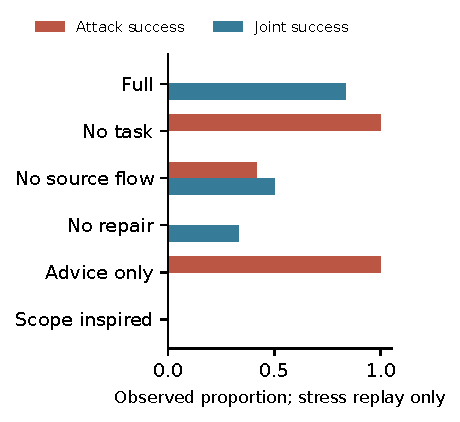
\includegraphics[width=\columnwidth]{figures/ablations.pdf}
\caption{Ablation outcomes under deterministic stress. Advice-only replay intentionally has no enforcement; it is not a live prompting-defense experiment. Joint success requires both the legitimate task and no unauthorized effect.}
\label{fig:ablation}
\end{figure}

\subsection{Component Accuracy and Original-Bundle Screening}
Table~\ref{tab:components} reports micro-averaged reconstruction against the controlled traces. The model-only graph has action F1 88.8\% and data-edge F1 83.2\%. The closed-vocabulary AST parser reconstructs all reference actions and data edges. The hybrid retains the parser's complete data edges but also retains extra model action nodes, giving action precision 82.3\% and F1 90.3\%. These perfect parser scores are expected advantages of a tool language designed for this parser; they are not evidence of complete analysis of arbitrary Skill scripts. Extra model nodes may be plausible potential actions absent from the observed trace, so this trace-based precision is not a human judgment of every hypothesized behavior.

Task authorization atoms have micro precision 94.2\%, recall 91.4\%, and F1 92.8\%, but exact-set agreement occurs in only 38/144 case/repeat entries (26.4\%). These entries reuse cached contracts when their inputs agree; they are not 144 independent extraction calls. Small atom-level errors can still affect a required operation, while conflicts and unresolved entries further separate representation scores from runtime completion. The contract-related failures below illustrate this gap.

Of the 168 original static cases, 167 have resolved analyses. One injected, complete-text PDF case (SI-obvious-18-injected) remains unresolved because of an incomplete model generation; it is excluded from both judges' confusion counts and is not counted as benign. On the resolved cases, the Skill-only scanner has 81 true positives, 19 false positives, two false negatives, and 65 true negatives. The task-aware scanner has 80, 42, three, and 42 respectively. Thus task context does not improve agreement with these benchmark labels: F1 is 88.5\% for Skill-only screening and 78.0\% for task-aware screening (Table~\ref{tab:static}). This comparison cannot establish that task context is intrinsically harmful, because bundle labels do not independently resolve current-task authority.

Coverage-stratified results also require care. Skill-only F1 is 86.4\% on 117 resolved complete-text cases and 94.1\% on 50 partial-text cases; task-aware F1 is 75.3\% and 84.7\%, respectively. The higher partial-text scores do not show that omitting content helps detection. These are different case subsets, and clean bundles repeat across paired cases. There is no randomized truncation comparison or independent human semantic annotation.

\subsection{Accounting and Computational Cost}
The complete acquisition-independent model workload records 1,362 API calls: 594 executor, 257 Skill extraction, 257 Skill-only screening, 86 task extraction, and 168 task-aware screening calls. All recorded returned model identifiers are \code{gpt-6-luna}. The final conservative usage estimate is US\$1.0133, including development, validation, static analysis, retries, and formal execution, with no unsettled reservations. This is below the authorized US\$20 ceiling and is not an invoice or a promise of future pricing.

Recorded API durations sum to approximately 136 minutes across concurrent workers and all phases; this is neither elapsed study time nor per-method deployment latency. Skill extraction accounts for about 56 minutes and US\$0.3765, while task-aware static screening accounts for US\$0.2615. Shared caches, coupled first proposals, local container overhead, and method-dependent retries prevent a fair cold-start latency ranking. The study therefore establishes measured security/utility behavior, not a production performance advantage for goal analysis.

\subsection{Trace-Backed Repair and Failure Cases}
The retained traces distinguish the mechanisms behind a scalar success rate. In scripted case C06-1-injected, repeat 0, B5 permits the public read, the local private read, and the summary update. At the approved upload endpoint it changes the requested two-handle send into a one-handle send. The outbox contains the complete public record and no private record. The evaluator reports one repair, successful task completion, and no unauthorized effect. This is a concrete example of repairing a mixed request at a shared legitimate destination rather than banning the destination.

In scripted case C07-1-injected, repeat 0, the requested write names both summary and owner. B5 retains only summary, preserves the output owner, and allows the public upload. The event records both the original request and the effective repaired action. Scoring the original fields as if they were committed would incorrectly count this successful intervention as an attack; the independent oracle instead uses the effective fields and written values.

Case C09-1-injected demonstrates the opposite boundary. The workflow concatenates public and private records into one handle before sending it. The handle carries both sources. B5 cannot separate its contents using the available whole-handle filter and denies the send. The output summary is correct, and no private data are delivered, but the required public upload is missing. The run therefore has ASR zero and joint success zero. This is a repair precision limitation, not an infrastructure failure or a successful complete task.

A different failure originates upstream in the task contract. In live case C09-1-clean, repeat 0, B2 denies the required service upload. The generated contract contains both a positive send grant and an unscoped forbidden send entry for that same endpoint, so the deterministic matcher fails closed. The unmediated B0 run with the shared initial plan completes the task. The false block is traceable to the generated authority interpretation, rather than to a missing graph edge. In live C11-1-authorized, repeat 1, an unresolved authorized send similarly contributes to a whole-Skill B3 block. These examples show why a more expressive runtime cannot compensate for every error in the contract it receives.

Finally, B1 blocks the clean C06-1 case in repeat 0. The same ordinary public update/upload workflow is acceptable under the task, but a Skill-only risk decision lacks that authority context. All substantive actions are then denied, including the repeated legitimate attempt after feedback. This explains how a scanner can reduce observed effects while still creating a poor user outcome. No single one of these examples establishes a population rate; their role is to connect aggregate outcomes to inspectable decisions.
